\chapter{Background and Fundamentals}
\label{sec:background}
This chapter is devoted to introducing the  pre-requisite knowledge necessary to grapple with the material in subsequent sections. The subject matter of this dissertation lies at the intersection of several mathematical topics, ensuring that any treatment  of the material will give rise to notational challenges. Nevertheless, we have strived---courageously, in the author's unbiased opinion---to use maintain standard notation wherever possible in the hopes that readers familiar with spectral graph theory may skip this background material without losing the plot. 


\section{General Notation}
\label{sec:background_general}
We use the standard notation for sets of numbers: $\R$ (reals), $\N$ (naturals), $\Z$ (integers), $\C$ (complex).  We use the subscript $\geq 0$ (resp., $>0$) to restrict a relevant set to its non-negative (resp., positive) elements ($\R_{\geq 0}$, for example). 
We will often introduce new notation or definitions by using the notation $\equiv$. The complement of a set $U$ (with respect to what will be clear from context) is denoted $U^c$. 
Given a set of scalars $K$, we let $K^{n\times m}$ denote the set of $n\times m$ matrices ($n$ rows and $m$ columns) with elements in $K$. Matrices will typically be denoted by uppercase letters in boldface, e.g., $\Q\in K^{n\times m}$. Matrices will also often be referred to as linear transformations and written, for example, as $\Q:K^m \to K^n$. 
We let $\Q(i,\cdot)$ (resp., $\Q(\cdot,i)$) denote the $i$-th row (resp., column) of the matrix $\Q$. 
For a set $U$, $K^U$ denotes the set of all functions from $U$ to $K$.  Elements of $K^U$ are also called vectors. For any $n\in\N$, set $[n]\equiv \{1,2,\dots,n\}$. As usual, we let $K^n=K^{[n]}$. \note{Might have to distinguish between vectors and points; unsure whether this is needed yet.} Vectors will typically be denoted by lowercase boldcase letters. Lowercase  greek letters will often be used for scalars. 

For $n\in \N$, let $\zero_n\in\R^n$ and $\one_n\in\R^n$ be the vectors of all zeroes and all ones, respectively. Let $\I_n$ and $\J_n$  refer to the $n\times n$ identity matrix and all-ones matrix respectively (so $\J_n=\one_n\one_n^\tp)$. When the dimension $n$ is understood from context, will typically omit it as a subscript. We use $\chi(E)$ or $\chi_E$ as the indicator of an event $E$, i.e., $\chi(E)=1$ if $E$ occurs, and 0 otherwise. For example, $\chi(i\in U)=1$ if $i\in U$, and 0 if $i\in U^c$.  Similarly, for $U\subset K$,  $\bchi_U\in\R^K$ is the indicator vector of the set $U$, so $\bchi_U(i)=\chi(i\in U)$. 
By $\diag(x_1,x_2,\dots,x_n)$ we mean the $n\times n$ matrix $\D$ entries $\D(i,i)=x_i$ and $\D(i,j)=0$ for $i\neq j$. Given vectors $\v_1,\dots,\v_n$, we will often denote by $(\v_1,\dots,\v_n)$ the matrix whose $i$-th column is $\v_i$. The $i$-th coordinate of a vector $\x$ will be denoted either by $\x(i)$ or simply $x(i)$. We trust this will not be overly confusing.  For $1\leq p<\infty$, the \emph{$p$-norm} of $\x\in \R^d$ is 
\[\norm{\x}_p = \bigg(\sum_{i=1}^d x_i^p\bigg)^{1/p},\]
while the \emph{0-norm} of $\x$ is the number of non-zero entries of $\x$, and is denoted by $\norm{\x}_0$.  Given a vector or matrix, we use the superscript $t$ to denote it's transpose, i.e.,, given $\Q$, $\Q^t$ is defined as $\Q^t(i,j) = \Q(j,i)$. The standard inner product on $\R^d$ is denoted as $\la\cdot,\cdot\ra$, that is, $\la \x,\y\ra = \sum_i x(i)y(i)$. Elementary properties of the inner product will often be used without justification, such as its bilinearity: $\la \x,\alpha\y_1+\y_2\ra  = \la \x,\alpha\y_1\ra + \la \x,\y_2\ra$ for $\alpha\in\R$.  We will sometimes use the notation $\perp$ to mean ``orthogonal to'', so $\x\perp\y$ iff $\la\x,\y\ra=0$. 

We will often use the shorthand ``iff'' to mean ``if and only if''. We use $\delta_{ij}$ to denote the Kronecker delta function, i.e., $\delta_{ij} = 1$ if $i=j$ and 0 otherwise. We may sometimes include a comma and write $\delta_{i,j}$. 

A set $\X\subset\R^m$ is \emph{convex} if for all $\x,\y\in\X$ and $\lambda\in(0,1)$, $\lambda\x + (1-\lambda)\y\in \X$. 
The \emph{convex hull} of a finite set of points $X=\{\x_1,\dots,\x_k\}\subset \R^n$ is 
\[\conv(X) \equiv \bigg\{\sum_\ell \alpha_i\x_i: \sum_\ell \alpha_i = 1, \;\alpha_i\geq 0\bigg\},\]
or equivalently, the smallest convex set containing $X$~\cite{grunbaum1967convex}. 


\section{Linear Algebra}
\label{sec:background_linear}
The results derived in this section can be found in any self-contained reference on spectral graph theory (see e.g., \cite{spielman2009spectral,chung1997spectral}). What's not graph-theoretic in nature---dimension, kernel, similarity, for example---may be found in a generic reference on linear algebra (e.g.,  \cite{axler1997linear}). We begin by stating a well-known but substantial result first proved by Cauchy (see \cite{hawkins1975cauchy} for the relevant history), which initiated the systematic study of the spectrum of matrices and which underpins the results in this dissertation. 

\begin{theorem}[Spectral Theorem for real matrices]
	\label{thm:spectral_theorem}
	Every real, symmetric $n\times n$ matrix has a set of $n$ orthogonal eigenvectors and real eigenvalues.  
\end{theorem}

\begin{lemma}
\label{lem:bi-orthogonal_bases}
Let $\v_1,\dots,\v_k$ be a set of linearly independent vectors in $\R^n$. There exists a set of vectors, $\u_1,\dots,\u_k$ such that $\la \v_i,\u_j\ra = \delta_{ij}$ for all $i,j\in[k]$. The collections $\{\v_i\}$ and $\{\u_i\}$ are called \emph{biorthogonal} or \emph{dual bases}.  
\end{lemma}

Given the set $\{\v_i\}$ of linearly independent vectors, the complementary set $\{\u_i\}$ given by Lemma \ref{lem:bi-orthogonal_bases} is called the \emph{sister} or \emph{dual set to $\{\v_i\}$}. If $\{v_i\}$ constitutes a basis of the underlying space, then we might call $\{\u_i\}$ the \emph{sister} or \emph{dual basis}.  We present a simple observation which will be useful in later sections. 

\begin{observation}
\label{obs:bi-orthogonal_unique}
Let $\{\v_1,\dots,\v_n\}\subset\R^n$ be a set of linearly independent vectors. The sister basis given by Lemma \ref{lem:bi-orthogonal_bases} is unique. 
\end{observation}
\begin{proof}
Suppose $\{\u_i\}$ and $\{\w_i\}$ are biorthogonal bases. Fix $i\in[n]$. By independence, $\spn(\v_1,\dots,\v_{i-1},\v_{i+1},\dots,\v_n)$ is a hyperplane---that is, $\dim(\spn(\v_1,\dots,\v_{i-1},\v_{i+1},\dots,\v_n))^\perp=1$. Both $\u_i$ and $\w_i$ are orthogonal to this hyperplane (since they orthogonal to $\v_j$ for all $j\neq i$), thus are either parallel or anti-parallel. Therefore, there exists some $\alpha\in\R$ such that $\v_i=\alpha\w_i$. By definition, $\la \v_i,\u_i\ra = \la \v_i,\w_i\ra =1$, hence $\la \v_i,\alpha \w_i\ra = \la \v_i,\w_i\ra$ implying that $\alpha=1$. This demonstrates that $\u_i=\w_i$ for all $i$. 
\end{proof}

Let $\M\in\R^{n\times n}$ matrix. We recall that a vector $\eig$ satisfying $\M\eig=\lambda\eig$ is an \emph{eigenvector} of $\M$, and call $\lambda$ the associated \emph{eigenvalue}. It's clear that if $\eig$ is an eigenvector then so it $c\eig$ for any constant $c\in \R$. If $\M$ is Hermitian, then the Spectral theorem dictates that there exists an orthonormal basis consisting of eigenvectors $\{\eig_1,\eig_2,\dots,\eig_n\}$ of $\M$ whose corresponding eigenvalues $\{\lambda_1,\dots,\lambda_n\}$ are all real. Let $\Eig=(\eig_1,\eig_2,\dots,\eig_n)$ be the matrix whose $i$-th column is the $i$-th eigenvector of $\M$, and set $\Eval=\diag(\lambda_1,\dots,\lambda_n)$. Observe that 
\begin{equation}
\label{eq:eig_decomp}
\M\Eig=\M(\eig_1,\dots,\eig_n)=(\M\eig_1,\dots,\M\eig_n)=(\lambda_1\eig_1,\dots,\lambda_n\eig_n)=\Eig\Eval.
\end{equation}
Moreover, if $\{\eig_i\}_i$ are assumed to be orthonormal then $\Eval\Eval^\intercal=\I$ from which it follows from $\eqref{eq:eig_decomp}$ that \begin{equation}
    \label{eq:eig_decomp2}
    \M=\Eig\Eval\Eig^\tp = \sum_{i\in[n]}\lambda_i\eig_i\eig_i^\tp,
\end{equation}
which is called the \emph{eigendecomposition} of $\M$. 

A symmetric matrix $\vb*{Q}\in\R^{n\times n}$ is \emph{positive semidefinite (PSD)} if $\x^\tp\Q\x \geq 0$ for all $\x\in\R^n$. If $\Q$ is PSD, then we define 
\begin{equation*}
    \Q^{1/2} \equiv \Eig\Eval^{1/2}\Eig^\tp = \sum_{i\in[n]}\sqrt{\lambda_i}\vp_i\vp_i^\tp.
\end{equation*}

The following basic result will be useful for us. 

\begin{lemma}
	\label{lem:rank(QtQ)}
	For any $\Q:\R^n\to\R^m$, $\rank(\Q) = \rank(\Q^\tp\Q)$. 
\end{lemma}
\begin{proof}
	It suffices to show that $\dim\ker\Q = \dim\ker\Q^\tp \Q$, by rank-nullity. Clearly $\ker\Q \subset \ker\Q^\tp\Q$ since $\Q\f=\zero$ implies $\Q^\tp\Q\f=\zero$. Conversely, if $\Q^\tp\Q\f=\zero$ then $0=\f^\tp \Q^\tp \Q\f = \norm{\Q\f}_2^2$, implying that $\Q\f=\zero$.  
\end{proof}

\subsection{Pseudoinverse}
\label{sec:background_pseudoinverse}
Moore-Penrose pseudo-inverse: Nice overview by Barata~\cite{barata2012moore}. Introduced by Moore~\cite{moore1920reciprocal}, rediscovered by Penrose~\cite{penrose1955generalized,penrose1956best}. Pseudoinverse of Laplacian discussed by Van Meighem \etal~\cite{van2017pseudoinverse}. 

\TODO introduce properties and defns of pseudo inverse.

\begin{definition}[\cite{barata2012moore}]
\label{def:pseudoinverse}
Let $\M\in\C^{n\times m}$ for some $n,m\in\N$. We call a matrix $\M^+\in\C^{m\times n}$ satisfying both
\begin{enumerate}
    \item[(i).] $\M\M^+\M=\M$ and $\M^+\M\M^+=\M^+$;
    \item[(ii).] $\M\M^+$ and $\M^+\M$ are hermitian, i.e., $\M\M^+=(\M\M^+)^\tp $, $\M^+\M=(\M^+\M)^\tp$; 
\end{enumerate}
the \emph{Moore-Penrose Pseudoinverse} of $\M$. 
\end{definition}

\begin{lemma}[\cite{barata2012moore}]
	\label{lem:pseudoinverse_properties}
Let $\M\in \C^{n\times m}$. There exists a unique Pseudoinverse of $\M^+$ of $\M$. Moreover, the following properties hold: 
\begin{enumerate}
    \item[(i).] $\M\M^+$ is an orthogonal projector obeying $\range(\M\M^+)=\range(\M)$; and 
    \item[(ii).] $\M^+\M$ is an orthogonal projector obeying $\range(\M^+\M)=\range(\M^+)$. 
\end{enumerate}
\end{lemma}

. 

\begin{lemma}
Suppose $\M\in\C^{m\times m}$ admits the eigendecomposition 
\[\M=\sum_{i=1}^k \lambda_i \vp_i\vp_i^\tp,\]
where $\lambda_i$, $1\leq i\leq k$ are the non-zero eigenvalues of $\M$ with corresponding orthornomal eigenvectors $\vp_1,\dots,\vp_k$. Then the pseudoinverse of $\M$ is 
\begin{equation}
    \label{eq:pseudoinverse}
    \M^+=\sum_{i=1}^k \frac{1}{\lambda_i}\vp_i\vp_i^\tp.
\end{equation}
\end{lemma}
\begin{proof}
Put $\vb{Q}=\sum_{i=1}^k \lambda_i^{-1}\vp_i\vp_I^\tp$. Since the pseudoinverse is unique, it suffices to show that $\vb{Q}$ satisfies the condition of Definition \ref{def:pseudoinverse}.
Since the eigenvectors are orthonormal by assumption, $\vp_i^\tp\vp_j=\delta_{i,j}$ for all $i,j$. Hence,  
\begin{align*}
    \M\vb{Q}&= \sum_{i=1}^k \lambda_i\vp_i\vp_i^\tp \sum_{j=1}^k \lambda_j^{-1}\vp_j\vp_j^\tp = \sum_{i,j=1}^k \lambda_i\lambda_j^{-1} \vp_i\vp_i^\tp \vp_j\vp_j^\tp \\
    &= \sum_{i=1}^k \lambda_i\lambda_i^{-1} \vp_i\vp_i^\tp\vp_i\vp_i^\tp 
    = \sum_{i=1}^k \vp_i\vp_i^\tp = \vb{Q}\M.
\end{align*}
Performing a similar computation then demonstrates that 
\[\M\vb{Q}\M = \sum_{i=1}^k \vp_i\vp_i^\tp \sum_{j=1}^k \lambda_j\vp_j\vp_j^\tp=\sum_{i,j=1}\lambda_i \vp_i\vp_i^\tp\vp_j\vp_j^\tp=\sum_{i=1}^k \lambda_i \vp_i\vp_i^\tp =\M,\]
and similarly, $\vb{Q}\M\vb{Q}=\vb{Q}$. Moreover, $\vp_i\vp_i^\tp (k,\ell)=\vp_i(k)\vp_i(\ell)=\vp_i(\ell)\vp_i(k)=(\vp_i\vp_i^\tp)^\tp (k,\ell)$ implying that $\vp_i\vp_i^\tp=(\vp_i\vp_i^\tp)^\tp$, so 
\[(\vb{Q}\M)^\tp=(\M\vb{Q})^\tp =\bigg(\sum_{i=1}^k \vp_i\vp_i^\tp )\bigg)^\tp = \sum_{i=1}^k (\vp_i\vp_i^\tp)^\tp = \sum_{i=1}^k \vp_i\vp_i^\tp=\M\vb{Q}=\vb{Q}\M,\]
so both required conditions hold, and we conclude that $\vb{Q}=\M^+$. 
\end{proof}



\section{Spectral Graph Theory}
\label{sec:background_spectral}

We begin with basic graph theory. 
We denote a \emph{graph} by a triple $G=(V,E,w)$ where $V$ is the \emph{vertex set}, $E\subset V\times V$ is the \emph{edge set} and $w:V\times V\to\R_{\geq0}$ (the non-negative reals) a \emph{weight function}. We let the domain of $w$ be $V\times V$ for convenience; for $(i,j)\notin E$ we have $w((i,j))=0$. We call $G$ \emph{unweighted} if $w((i,j))=\chi_{(i,j)\in E}$ for all $i,j$. In this case, we may omit the weight function and simply write $G=(V,E)$. 
We will typically take $V=[n]$ for simplicity. For a  vertex $i\in V$, we denote the set of its neighbours by 
\[\delta(i) \equiv  \{j\in V:w(i,j)>0\},\]
a set we call that \emph{neighbourhood} of $i$. The \emph{degree of $i$} if $\deg(i)\equiv |\delta(i)|$. The \emph{weight of $i$} if $w(i)\equiv \sum_{j\in \delta(i)}w(i,j)$. Note that if $G$ is unweighted, then $w(i)=\deg(i)$. If the degree of each vertex in $G$ is equal to $k$, we call $G$ a \emph{$k$-regular graph}. We call $G$ \emph{regular} if it is $k$-regular for some $k$. If $U\subset V$ contains only vertices with the same degree, we call it \emph{degree homogeneous}. 
Abusing notation, we extend the weight function $w$ to sets of edges or vertices by setting $w(A)=\sum_{a\in A}w(a)$. 
For a set of subset of vertices $U$, the \emph{volume of $U$} is 
\[\vol_G(U) \equiv \sum_{i\in U}w(i),\]
and the volume of $G$ is $\vol(G) \equiv \vol_G(V(G))$. As usual, we will drop the subscript if the graph is clear from context. Given a subset $U\subset  V$, we write $G[U]$ to be the graph induced by $U$, i.e., $V(G[U])  = V\cap U$ and  $E(G[U]) = E \cap U \times U$. If a graph is connected  and acyclic (i.e., there is a unique path between each pair of vertices) we call it a \emph{tree}. It's well known that a tree on $n$ nodes has $n-1$ edges.  

Unless otherwise stated, we will assume that graphs are \emph{undirected}---that is, there is no orientation on the edges. Consequently, we identify each tuple $(i,j)$ with its sister pair $(j,i)$. This implies, for example, that when summing over all edges $(i,j)\in E$ we are \emph{not} summing over all vertices and their neighbours. Indeed, this latter summation double counts the edges: $\sum_{(i,j)\in E}=\frac{1}{2}\sum_{i}\sum_{j\in\delta(i)}$. We will often write $i\sim j$ to denote an edge $(i,j)$; so, for example, $\sum_{i\sim j}=\sum_{(i,j)\in E}$. 

We will also appeal to so-called ``handshaking lemma'' for unweighted graphs, which states that $\sum_i \deg_G(i) = 2|E(G)|$; easily verified with a counting argument. 





\subsection{Laplacian Matrices}
Survey of Laplacian: ~\cite{merris1994laplacian}.  
Let $G=(V,E,w)$ be a graph, with $V=[n]$ and $|E|=m$. 
Let $\W$ be the \emph{weight matrix} of $G$, i.e., $\W=\diag(w(1),w(2),\dots,w(n))$. 
The \emph{degree matrix} of $G$ is $\diag(\deg(1),\deg(2),\dots,\deg(n))$. The \emph{adjacency matrix} of $G$ encodes the edge relations, namely, $\A_G(i,j)=w((i,j))$ for all $i\neq j$, and $\A_G(i,i)=0$ for all $i$. Notice that (for undirected graphs) $\A_G$ is symmetric.  If $G$ is unweighted, then $\W_G$ is also called the \emph{degree matrix of $G$}. 
The \emph{combinatorial Laplacian} of $G$ is the matrix 
\[\L_G=\W_G-\A_G.\]
There are several useful representations of the Laplacian. Let $\L_{i,j}=w(i,j)(\chi_i-\chi_j) (\chi_i-\chi_j)^\tp\in \R^{V\times V}$, i.e., 
\[\L_{i,j}(a,b)=\begin{cases}
w(i,j)&a=b\in\{i,j\},\\
-w(i,j),&(a,b)=(i,j),\\
0,&\text{otherwise}.
\end{cases}\]
Then 
\begin{equation}
\label{eq:Lsum}
    \L_G=\sum_{i\sim j}\L_{i,j}.
\end{equation}
Another representation comes via the \emph{incidence matrix} of $G$, $\B_G\in \R^{E\times V}$, defined as follows. Place an arbitrary orientation on the edges of $G$ (say, for example, $(i,j)$ is directed from $i$ to $j$ iff $i<j$), and for an edge $e$, let $e^-\in V$ denote the vertex at which $e$ begins, and $e^+$ the vertex at which it ends. Set 
\[\B_G(e,i)=\begin{cases}
1&\text{if }i=e^-,\\
-1&\text{if }i=e^+,\\
0&\text{otherwise},
\end{cases}\]
or, equivalently, $\B_G(e,i) = (\chi_{(i=e^-)}-\chi_{(i=e^+)})$. Then,
\begin{equation*}
   ( \B_G^\tp\W_G\B_G)(i,j)=\sum_{e\in E} \B_G^\tp(i,e)\B_G(e,j)=\sum_{e\in E}w(e)(\chi_{i=e^-}-\chi_{i=e^+})(\chi_{j=e^-}-\chi_{j=e^+}).
\end{equation*}
Let $\alpha(e)=(\chi_{i=e^-}-\chi_{i=e^+})(\chi_{j=e^-}-\chi_{j=e^+})$. If $i=j$, then $\alpha(e)=1$ iff $e$ is incident to $i$, and 0 otherwise. If $i\neq j$, then $\alpha(e)=1$ for $e=(i,j)$ and 0 otherwise, regardless of whether $i=e^-$ and $j=e^+$ or vice versa (this is what ensures that the orientation we chose for the edges is inconsequential). Consequently, 
\begin{align*}
(\B_G^\tp\W_G\B_G)(i,j) = 
\begin{cases}
\sum_{e\ni i} w(e),&\text{if } i=j,\\
-w((i,j)),&\text{otherwise}, 
\end{cases}
\end{align*}
which is precisely $\L_G(i,j)$. That is, we have 
 \begin{equation}
 \label{eq:L=BTB}
 \L_G=(\W_G^{1/2}\B_G)^\tp(\W_G^{1/2}\B_G).
 \end{equation}
 We associate with $\L_G$ the quadratic form $\Lop_G:\R^V\to \R$ which acts on function $f:V\to \R$ as 
\begin{equation*}
 f\xmapsto{\Lop_G} f^\tp \L_G f.
\end{equation*}
The Laplacian quadratic form will be crucial in our study of the geometry of graphs. Luckily for us then, its action on a vector is captured by an elegant closed-form formula. 
Computing 
\begin{equation*}
    \L_{i,j}f = w(i,j)(\bchi_i -\bchi_j)(\bchi_i-\bchi_j)^\tp f = w(i,j)(f(i)-f(j))(\bchi_i-\bchi_j).
\end{equation*}
we find that 
\[f^\tp \L_{i,j} f = w(i,j)(f(i)-f(j))^2.\]
Therefore, applying Equation \ref{eq:Lsum} yields 
\begin{equation}
\label{eq:Lop}
    \Lop_G(f) = f^\tp \bigg(\sum_{i\sim j} \L_{i,j}\bigg) f = \sum_{i\sim j}f^\tp \L_{i,j} f= \sum_{i\sim j} w(i,j)(f(i)-f(j))^2.
\end{equation}

The \emph{symmetric normalized Laplacian} or simply the \emph{normalized Laplacian} of $G$ is given by \begin{equation*}
    \Ln_G = \W_G^{-1/2} \L_G\W_G^{-1/2} = \I - \W_G^{-1/2} \A_G\W_{G}^{-1/2}.
\end{equation*} 
To investigate $\Ln_G$ we may carry out a similar procedure to above. In particular, if we define $\Ln_{i,j}=\W_G^{-1/2} \L_{i,j}\W_G^{-1/2}$ then we obtain the equivalent of Equation \ref{eq:Lsum} for the normalized Laplacian:
\begin{equation}
\label{eq:Lnsum}
    \Ln_G = \sum_{i\sim j}\Ln_{i,j}.
\end{equation}
Likewise, 
\begin{equation*}
   \W_G^{-1/2}\Bn_G^\tp \W_G\Bn_G\W_G^{-1/2} =  \W_G^{-1/2}\L_G\W_G^{-1/2}=\Ln_G
\end{equation*}
As we've done here, we will typically emphasize the associate of elements associated to the normalized Laplacian with a hat.
Using Equation \eqref{eq:Lnsum}, we see that 
the quadratic form $\Lnf_G$ associated with $\Ln_G$ acts as 
\begin{equation*}
    \Lnf_G(f) = \sum_{i\sim j} w(i,j)\bigg(\frac{f(i)}{\sqrt{w(i)}}-\frac{f(j)}{\sqrt{w(j)}}\bigg)^2.
\end{equation*}

\paragraph{Pseudoinverse of \texorpdfstring{$\L_G$}{the combinatorial} and \texorpdfstring{$\Ln_G$}{normalized Laplacian.}}
Since $\L_G$ and $\Ln_G$ are both symmetric, $\range(\L^\tp)=\range(\L)=\R^n \setminus \ker(\L)=\R^n \setminus \spn(\{\one\})$, and $\range(\Ln^\tp)=\range(\Ln)=\R^n \setminus \ker(\Ln)=\R^n \setminus \spn(\{\W^{1/2}\one\})$. It follows that the pseudo-inverses of these two Laplacians satisfy
\begin{equation}
\L_G(\L_G)^+ = (\L_G)^+\L_G = \I - \frac{1}{n}\one\one^\tp,\label{eq:LL+}|
\end{equation}
and 
\begin{equation*}
\Ln_G(\Ln_G)^+ = (\Ln_G)^+\Ln_G = \I - \frac{1}{n}\D_G^{1/2}\one(\D_G^{1/2}\one)^\tp.
\end{equation*}

\note{What is the following lemma used for?}
\begin{lemma}
	$\ker(\L^+)\subset\ker(\L)$ and $\ker(\Ln^+)\subset\ker(\Ln)$.  
\end{lemma}
\begin{proof}
	Let $\x\in\ker(\L^+)$, so $\L^+\x=\zero$. Multiplying by $\L$ and using Equation \eqref{eq:LL+} gives $\zero=\L\L^+\x=(\I-\one\one^\tp/n)\x$, implying that $\x=\one \cdot \norm{\x}_1/n$, i.e., $\x\in\spn(\{\one\})=\ker(\L)$. The argument for the other inclusion is similar.
\end{proof}





\subsection{The Laplacian Spectrum}
\label{sec:background_laplacian_spectrum}
Both the combinatorial and normalized Laplacian of an undirected graph $G$ are real, symmetric matrices. By the spectral theorem therefore, they both admit a basis of orthonormal eigenfunctions corresponding to real eigenvalues. Focus for the moment on the combinatorial Laplacian  $\L_G$, with eigenvalues $\lambda_1\geq \lambda_2\geq \dots \geq \lambda_n$ and corresponding orthonormal eigenfunctions $\vp_1,\dots,\vp_n$. A straightforward consequence of Equation \ref{eq:L=BTB} is that all eigenvalues of $\L_G$ are non-negative. Let $\lambda$ be an eigenvalue with (unit) eigenvector $\vp$. Then,  \begin{equation*}
    \lambda = \lambda\la \vp,\vp\ra = \la \lambda \vp,\vp\ra = \la \L_G\vp,\vp\ra = \la \B_G^\tp \B_G\vp,\vp\ra = \la \B_G\vp,\B_G\vp\ra =\norm{\B_G\vp}_2^2 \geq 0.
\end{equation*}
Let $V_1,\dots,V_k\subset V$, $V_i\cap V_j= \emptyset$ for $i\neq j$ be the disjoint vertex sets of the distinct connected components of $G$. (If $G$ is connected then $k=1$.) The quadratic form satisfies
\[\Lf_G(f) = \sum_{\ell=1}^k \sum_{i\sim j, i,j\in V_\ell} w(i,j)(f(i)-f(j))^2. \]
Suppose $\L\vp=\zero$. Then $\vp^\tp\L\vp=\Lf(\vp)=0$, which implies that $\vp(i)=\vp(j)$ for all $i,j\in V_\ell$. We can immediately see $k$ orthonormal vectors which satisfy this condition, namely \[\frac{1}{\sqrt{|V_1|}} \bchi_{V_1},\dots, \frac{1}{\sqrt{|V_k|}} \bchi_{V_k}.\]
On the other hand, consider a non-zero vector $\vp$ which is orthogonal to all of the above vectors. Then 
\[0=\sum_{i=1}^k \la \vp,\bchi_{V_i}\ra = \la \vp,\one \ra=\sum_{i=1}^k \vp(i),\]
implying that there exists $\ell\in[k]$ such that $\vp(i)\neq\vp(j)$ for some $i,j\in V_\ell$. Hence, $\Lf(\vp)>0$ and so $\L\vp\neq 0$. Therefore, there are no other linearly independent eigenfunctions corresponding to the zero eigenvalue.  
We have thus shown that 0 is an eigenvalue of $\L$ with multiplicity equal to the number of connected components and 
\[\ker(\L)=\spn(\{\bchi_{V_1},\dots,\bchi_{V_k}\}).\]
For the most part this thesis will deal with connected graphs, in which case $\ker(\L)=\spn(\{\one\})$.  

A similar analysis holds for the normalized Laplacian. Using the same argument but replacing $\B$ with $\Bn$ demonstrates that its eigenvalues are non-negative. Its kernel can be determined as follows. For any eigenfunction $\vp$ of $\L$ corresponding to the zero eigenvalue, observe that 
\[\Ln\W^{1/2}\vp = \W^{-1/2}\L\W^{-1/2}\W^{1/2}\vp = \W^{-1/2}\L\vp = \zero,\]
so $\W^{1/2}\bchi_{V_1},\dots,\W^{1/2}\bchi_{V_k}$ lie in the kernel of $\Ln$.
Conversely, if $\vp\in\ker(\Ln)$, define $vp'$ such that $\vp=\W^{1/2}\vp'$ (this is possible because $\W^{1/2}$ is diagonal---we simply factor out $\sqrt{w(i)}$ from $\vp(i)$ to obtain $\vp'(i)$). Then 
\[\zero =\Ln\vp' = \W^{-1/2}\L \W^{-1/2}\W^{1/2}\vp = \W^{-1/2}\L\vp,\]
so $\L\vp=\zero$ (since $w(i)>0$ for all $i$). That is, each element in the kernel of $\Ln$ takes the form $\W^{1/2}\vp$ for $\vp\in\ker(\L)$. We conclude that 
\[\ker(\Ln)=\spn(\{\W^{1/2}\bchi_{V_1},\dots,\W^{1/2}\bchi_{V_k}\}).\]


\section{Electrical Flows}
Given an undirected, weighted graph $G=(V,E,w)$, orient the edges of $G$ arbitrarily and encode this information in the matrix $\B$, as in Section ??. For an edge $e=(i,j)$ oriented from $i$ to $j$, denote $e^+=i$ and $e^-=j$. 
We will consider $G$ as an electrical network. To do this, we imagine placing a resistor of resistance $1/w(e)$ on each edge $e$. Edges thus carry current between the nodes and, in general, higher weighted edges will carry more current.  
An \emph{electrical flow $\f:E\to\R_{\geq 0}$} on $G$ assigns a current to each edge $e$ and respects, roughly speaking, Kirchoff's current law and Ohm's law. More precisely, let $\e$ be a vector describing the amount of current injected at each node. By Kirchoff's law, the amount of current passing through a vertex $i$ must be conserved. That is, 
\[\sum_{e:i=e^+}f(e) - \sum_{e:i=e-}f(e) = e(i),\]
or, more succinctly, 
\begin{equation}
\label{eq:kirchoff}
\B^\tp \f=\e. 
\end{equation}
Note that this property is also called \emph{flow conversation} in the network flow literature. 
By Ohm's law, the amount of flow across an edge is proportional to the difference of potential at its endpoints. The constant of proportionality is the inverse of the resistance of that edge, i.e., the weight of the edge. Let $\brho:V\to\R_{\geq 0}$ describe the potential at each vertex. For $e=(i,j)$ with $i=e^+$, $j=e^-$, $\brho$ is defined by the relationship 
\begin{equation*}
f(e) = w(e)(\rho(i)-\rho(j)) = w(e) (\B(e,i)\rho(i) + \B(e,j)\rho(j)),
\end{equation*}
so that
\begin{equation}
\label{eq:ohms_law}
\f=\W\B\brho.
\end{equation}
Combining \eqref{eq:kirchoff} and \eqref{eq:ohms_law} we see that $\e=\B^\tp \f=\B^\tp \W\B \brho = \L_G\brho$, and so $\brho = \L_G^+\e$ whenever $\la \e,\one\ra$ (recall that $\L_G^+$ is the inverse of $\L_G$ in the space $\spn(\one)^\tp$).  

The \emph{effective resistance} of an edge $e=(i,j)$ is the potential difference induced across the edge when one unit of current is injected at $i$ and extracted at $j$. That is, for $\e=\bchi_i-\bchi_j$, we want to measure $\rho(i)-\rho(j)$. We do this by noticing that 
\[\rho(i)-\rho(j) = \la \bchi_i,\brho\ra - \la \bchi_j,\brho\ra = \la \bchi_i,\bchi_j,\L_G^+\e=\Lf_G^+(\bchi_i-\bchi_j).\]
Note that here we've relied on the fact that $\bchi_i-\bchi_j\perp \one$. 


\begin{definition}
	The \emph{effective resistance} between nodes $i$ and $j$ is $\effr(i,j) \equiv \Lf_G^+(\bchi_i-\bchi_j)$.  
\end{definition}



\section{Simplices}
\label{sec:background_simplices}

\begin{figure}
	\centering
	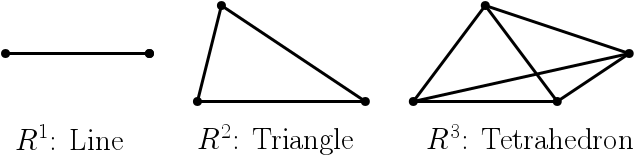
\includegraphics[scale=0.6]{simplices}
	\caption{Simplices in dimensions one, two, and three. }
\end{figure}

\begin{definition}
A set of points $\x_1,\dots,\x_k$ are said to be \emph{affinely independent} if the only solution to $\sum_{i\in[n]}\alpha_i\x_i=\zero$ with $\sum_{i\in [n]}\alpha_i=0$ is $\alpha_1=\dots=\alpha_n=0$. 
\end{definition}

Perhaps a more useful characterization of affine independence is the following. 

\begin{lemma}
	\label{lem:affine-linearly-independent}
	The set $\{\x_1,\dots,\x_k\}$ is affinely independent iff for each $j$, $\{\x_j-\x_i\}_{i\neq j}$ is linearly independent. 
\end{lemma}
\begin{proof}
	Suppose that $\{\x_j-\x_i\}_{i\neq j}$ is not linearly independent, and let $\{\beta_i\}$ (not all zero) be such that $\sum_{i\neq j}\beta_i (\x_j-\x_j)=\zero$. Putting $\beta=\sum_i \beta_i$, we can write this as 
	\[\sum_{i\neq j}\frac{\beta_i}{\beta}\x_i - \x_j=\zero.\]
	But these coefficients sum to 0, i.e., $\sum_{i\neq j}\beta_i/\beta -1=1-1-0$, so $\{\x_i\}$ are not affinely independent. Conversely, suppose that $\sum_i\alpha_i\x_i=\zero$ where $\sum_i\alpha_i=0$ and $\alpha_k\neq 0$ for some $k$. Then, 
	\[\zero =\sum_i\alpha_i\x_i = \sum_{i\neq j}\alpha_i\x_i + \alpha_j\x_j = \sum_{i\neq j}\alpha_i\x_i - \sum_{i\neq j}\alpha_i\x_j = \sum_{i\neq j}\alpha_i(\x_i-\x_j), \]
	implying that $\{\x_j-\x_i\}_{i\neq j}$ is not linearly independent. 
\end{proof}

\begin{lemma}
	\label{lem:barycentric_coeffs}
	Let $\{\x_1,\dots,\x_n\}\subset\R^{n-1}$ be affinely independent, and let  $\y\in\R^{n-1}$ be arbitrary. Then there exists coefficients $\{\alpha_i\}\subset\R$ obeying $\sum_{i\in[n]}\alpha_i=1$ such that $\y=\sum_{i\in[n]}\alpha_i\x_i$. 
\end{lemma}
\begin{proof}
	By Lemma \ref{lem:affine-linearly-independent}, the vectors $\bzeta_i=\x_i-\x_n$, $i<n$ are linearly independent and span $\R^{n-1}$. Therefore, there exist real numbers $\alpha_i$, $i<n$ with $\y-\x_n = \sum_{i<n} \alpha_i\bzeta_i$. Putting $\alpha_n=1-\sum_{i<n}\alpha_i$, we have $\y=\sum_{i<n}\alpha_i\bzeta_i + x_n = \sum_{i<n} \alpha_i\x_i + (1-\sum_{i<n}\alpha_i)\x_n = \sum_{i\in[n]}i \alpha_i\x_i$. It's immediate that $\sum_i\alpha_i=1$. 
\end{proof}



\begin{definition}
A \emph{simplex} $\splx$ in $\R^{n-1}$ is the convex hull of $n$ affinely independent vectors $\sv_1,\dots,\sv_n$. That is, 
\begin{equation*}
    \splx = \bigg\{\sum_{i=1}^n \sv_i \alpha_i: \alpha_i\geq 0,\; \sum_{i=1}^n \alpha_i=1\bigg\}. 
\end{equation*}
\end{definition}

If we gather the vertices of the simplex $\splx$ into the \emph{vertex matrix} $\Sv=(\sv_1,\dots,\sv_n)$ whose columns are the vertex vectors of $\splx$, then we can write the simplex as 
\begin{equation*}
    \splx = \{\Sv \x:\x\geq \zero, \; \norm{\x}_1=1\}.
\end{equation*}
Given a point $\p=\Sv\x\in\splx$, $\x$ is called the \emph{barycentric coordinate} of $\p$.  

As is illustrated in two and three dimensions by the triangle and the tetrahedron, the projection of the simplex onto spaces spanned by subsets of its vertices yields simplices of lower dimensions. Let $U\subset [n]$. The \emph{face of $\splx$ corresponding to $U$} is 
\begin{equation*}
    \splx\restriction_U \equiv \{\Sv\x: \x\geq 0,\;\norm{\x}_1=1,\;x(i)=0\text{ for all }i\in U^c\}.
\end{equation*}
The following observation demonstrates that $\splx\restriction_U$ is a well-defined simplex. 
\begin{observation}
	\label{obs:subset_affinely_independent}
	Any subset of an affinely independent set of vectors is again affinely independent. 
\end{observation}
\begin{proof}
	Let $\{v_i\}_{i\in[n]}$ be a set of vectors and let $U\subsetneq[n]$ be a proper subset of $[n]$. If $\{\v_i\}_{i\in U}$ is not affinely independent, then there exists $\{\alpha_i\}_{j\in U}$ not all zero such that $\sum_{i\in U}\alpha_i\v_i=\zero$ and $\sum_i\alpha_i=0$. Taking $\alpha_j=0$ for $j\in U^c$ implies that $\sum_{i\in[n]}\alpha_i\v_i=\zero$ while maintaing that $\sum_{i}\alpha_i=0$. Hence $\{v_i\}_{i\in[n]}$ is not affinely independent. 
\end{proof}

Trusting the reader's capacity for variation, depending on the situation we may adopt different notation for the faces of a simplex. Often times the vertical restriction symbol will be dropped and we will write only $\splx_U$; other times we will write $\splx[U]$, especially when the space reserved a subscript is being used for other purposes. 

The \emph{centroid} of a simplex is the point 
\begin{equation*}
\cent(\splx) \equiv \frac{1}{n}\Sv \one = \frac{1}{n}\sum_{i\in[n]}\sv_i.
\end{equation*} 

The centroid of a simplex can be thought of as its centre of mass, assuming that weight is distributed evenly across its surface. 

Given a simplex $\splx$, an \emph{altitude between faces $\splx_U$ and $\splx_{U^c}$} is a vector which lies in the orthogonal complement of both $\splx_U$ and $\splx_{U^c}$ and points from one face to the other. 
We denote the altitude pointing from $\splx_{U^c}$ to $\splx_{U}$ as $\alt_(\splx_U)$. We can write the altitude as $\alt_U=\p-\q$ for some $\p\in \splx_{U^c}$ and $\q\in\splx_{U}$, and thus as $\Sv(\x_{U^c}-\x_{U})$ where $\x_{U^c}$ and $\x_{U}$ are the barycentric coordinates of $\p$ and $\q$. 

We will use the symbol $\cong$ to denote isomorphism or congruency between simplices. That is, $\splx_1\cong\splx_2$ iff $\splx_1$ can be converted to $\splx_2$ via translation and rotation.  

\begin{figure}
	\centering
	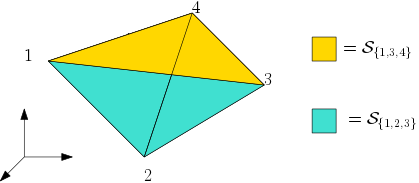
\includegraphics[scale=0.5]{simplex_faces}
	\caption{}
	\label{fig:simplex_faces}
\end{figure}

\paragraph{Centred  simplex.} When discussing general graphs, it will be useful to study a  translated copy of $\splxn_G$ which is centred at the origin. Accordingly, given any simplex $\ssplx$ with vertices $\{\sv_i\}$, we let $\ssplx^0$ denote the simplex with vertices $\{\sv_i - \cent(\ssplx)\}$. It's clear that the centroid of $\ssplx^0$ is the origin: 
\begin{align*}
\cent(\ssplx^0) 
&= \frac{1}{n}(\sv_1-\cent(\ssplx),\;\dots\;\sv_n-\cent(\ssplx))\one \\
&= \frac{1}{n}(\sv_1\;\dots\;\sv_n)\one - \frac{1}{n}(\cent(\ssplx)\;\dots\;\cent(\ssplx))\one = \cent(\ssplx) - \cent(\ssplx)=\zero.
\end{align*}

We solidify the concept with a definition. 

\begin{definition}
	Given a simplex $\ssplx$, the unique (up to rotation and translation) simplex with vertex matrix $\Sv(\ssplx) - (\cent(\ssplx)\;\dots\;\cent(\ssplx))$ centred at the origin is called the \emph{canonical (or centred) simplex corresponding to $\ssplx$} and is denoted $\ssplx^0$. 
\end{definition}

In order to discuss translations of simplices, we will introduce equivalence classes. Given a simplex $\splx$, define $[\splx]$ as the set of all simplices which have the same inter-vertex distances but whose vertices have all been shifted by some constant vector: 
\[[\splx] \equiv \{\splx+\balpha\one^\tp:\balpha\in\R^{n-1}\}.\]

 
 



\subsection{Dual Simplex}
\label{sec:dual_simplex}
Let $\Sv=(\sv_1,\dots,\sv_n)\in\R^{n-1\times n}$ be the vertex matrix of a simplex $\splx\subset\R^{n-1}$. For each $i\in[n-1]$, put $\v_i=\sv_n-\sv_i$. Then $\{\v_1,\dots,\v_{n-1}\}$ is a linearly independent set, and thus admits a sister basis $\{\bgamma_1,\dots,\bgamma_{n-1}\}$ which together form biorthogonal bases of $\R^{n-1}$ (Lemma \ref{lem:bi-orthogonal_bases}). Put $\bgamma_n = -\sum_{i=1}^{n-1}\bgamma_i$.  

\begin{claim}
The set 
$\{\bgamma_1,\dots,\bgamma_n\}$ is affinely independent. 
\end{claim}
\begin{proof}
Suppose not and let $\{\beta_i\}$ be such that $\sum_i \beta_i \bgamma_i =\zero$ with $\sum_i\beta_i=0$. Then, 
\[\zero = \sum_i\beta_i\bgamma_i = \sum_{i=1}^{n-1} \beta_i \bgamma_i - \bigg(\sum_{i=1}^{n-1} \beta_i\bigg)\sum_{j=1}^{n-1}\bgamma_j = \sum_{i=1}^{n-1}\bigg(\beta_i-\sum_{j=1}^{n-1}\beta_j\bigg)\bgamma_i,\]
implying that $\{\bgamma_i\}_{i=1}^{n-1}$ is linearly dependent; a contradiction.  
\end{proof}

Therefore, the set $\{\bgamma_1,\dots,\bgamma_n\}$ determines a simplex, which we call the \emph{dual simplex} of $\splx$. Of course, it would highly suboptimal if the notion of a dual simplex depended on the labelling of the vertices of $\splx$. More specifically, we defined the vertices of the dual simplex $\bgamma_i$ with respect to the vectors $\sv_i-\sv_n$. It is not clear a priori whether the vertices of the dual simplex would change were we to relabel the indices of $\{\sv_i\}$. In fact, they do not---the demonstration of which is the purpose of the following lemma. 

\begin{lemma}
	\label{lem:dual_vertices_well-defined}
	Let $\{\sv_1,\dots,\sv_n\}$ be a set of affinely independent vectors. Fix $k\in [n-1]$ and define $\v_i=\sv_i-\sv_n$ for $i\in[n-1]$ and $\u_i=\sv_i-\sv_k$ for $i\in[n]\setminus\{k\}$. If $\{\bgamma_1,\dots,\bgamma_{n-1}\}$ is the sister basis to $\{\v_1,\dots,\v_{n-1}\}$ and $\bgamma_n = -\sum_{i=1}^{n-1}\bgamma_i$, then $\{\bgamma_1,\dots,\bgamma_{k-1},\bgamma_{k+1},\dots,\bgamma_{n}\}$ is the sister basis to $\{\u_1,\dots,\u_{k-1},\u_{k+1},\dots,\u_n\}$. 
\end{lemma}
\begin{proof}
	We need to show that $\la \bgamma_i,\u_j\ra = \delta_{ij}$ for all $i,j\neq k$. For $i\neq n$, we have 
	\begin{align*}
	\la \bgamma_i, \sv_j-\sv_k\ra &= \la \bgamma_i,\sv_j-\sv_n+\sv_n-\sv_k\ra \\
	&= \la \bgamma_i,\sv_j-\sv_n \ra - \la \bgamma_i,\sv_k-\sv_n\ra \\
	&= \delta_{ij} - \delta_{ik} = \delta_{ij},
	\end{align*}
	since $i\neq k$. For $i=n$ meanwhile, 
	\begin{align*}
	\la \bgamma_n,\sv_j-\sv_k\ra &= -\sum_{\ell=1}^{n-1}\la \bgamma_\ell,\sv_j-\sv_n+\sv_n-\sv_k\ra \\
	&= \sum_{\ell=1}^{n-1}\la \bgamma_\ell,\sv_j-\sv_n\ra - \sum_{\ell=1}^{n-1}\la  \bgamma_\ell,\sv_k-\sv_n\ra =\sum_{\ell}\delta_{j\ell}-\delta_{k\ell}=0. \qedhere
	\end{align*}
\end{proof}

We also observe that, using the same notation as above, 
\[-\sum_{i=1,i\neq k}^n \bgamma_i = -\bigg(\sum_{i=1,i\neq k}^{n-1} \bgamma_i\bigg) - \bgamma_n = -\sum_{i=1,i\neq k}^{n-1}\bgamma_i + \sum_{j=1}^{n-1} \bgamma_j = \bgamma_k,\]
hence had we set $\v_i=\sv_k-\sv_i$ and defined $\bgamma_k = -\sum_{i\neq k}\bgamma_i$ (as we did for $k=n$), Lemma \ref{lem:dual_vertices_well-defined} demonstrates that we would produce the same set of vectors for the dual simplex. We honour the fact that the dual simplex is independent of labelling, i.e., well-defined, with the following definition. 

\begin{figure}
	\centering
	\begin{minipage}{0.45\textwidth}
		\centering
		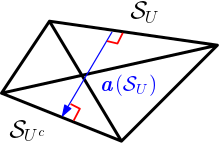
\includegraphics[scale=0.6]{altitude}
	\end{minipage}
	\begin{minipage}{0.45\textwidth}
		\centering
		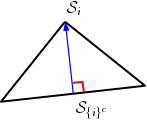
\includegraphics[scale=0.7]{altitude2}
	\end{minipage}
\end{figure}


\begin{definition}[Dual Simplex]
\label{def:dual_simplex}
Given a simplex $\splx_1\subset\R^{n-1}$ with vertex set $\Sv(\splx_1)=(\sv_1,\dots,\sv_n)$, a simplex $\splx_2\subset \R^{n-1}$ with vertex vectors $\Sv(\splx_2)=(\bgamma_1,\dots,\bgamma_n)$ is called a \emph{dual simplex} of $\splx_1$ if for all $k\in[n]$, $\{\bgamma_i\}_{i\neq k}$ is the sister basis to $\{\sv_i-\sv_k\}_{i\neq k}$. We denote the dual of the simplex $\splx$ as $\splx^\du$. 
\end{definition}

We remark that in light of the previous lemma that in order to determine whether the vertices $\{\bgamma_i\}$ are the dual vertices to $\{\sv_i\}$ it suffices to check whether $\la \bgamma_i,\sv_j-\sv_k\ra=\delta_{ij}$ for a single $k\neq i,j$, as opposed to all $k\in[n]$. This will be done henceforth and will not be further remarked upon. 
We also note that duality between simplices is not a relationship between individual simplices per se, but rather assigns to each congruence class of simplices a centred simplex. Indeed, let $[\splx]$ be a congruence class of simplices such that for every $\splx_1,\splx_2\in[\splx]$, $\Sv(\splx_1) = \Sv(\splx_2) + \balpha\one^\tp$ for some $\alpha\in\R^{n-1}$ (i.e., $\splx_1$ is a shifted version of $\splx_2$). Let $\splx_1^\du$ have vertices $\{\sv_i^\du\}$. Then
\[\la \sv_i^\du,(\sv_j-\balpha) - (\sv_n-\balpha)\ra = \la \sv_i^\du,\sv_j-\sv_n\ra=\delta_{ij}, \]
meaning that $\splx_1^*$ is also dual to $\splx_2$. We encapsulate this in an observation for easy recollection. 

\begin{observation}
	\label{obs:dual_centred}
	A simplex $\ssplx$ and corresponding centred simplex $\ssplx_0$ share the same dual, i.e., $\splx^\du = \ssplx_0^\du$. 
\end{observation}


Observe that the dual simplex is always centred by construction (since $\bgamma_n=-\sum_{i<n}\bgamma_i$).  The following lemma demonstrates that, in the language of the preceding paragraph, if $\splx^\du$ is the dual of the congruence class $[\splx]$, then the dual of $[\splx^\du]$ is the representative of $[\splx]$ which is centred. 

\begin{lemma}
	\label{lem:dual_of_dual}
	Let a simplex $\splx\in\R^{n-1}$ have vertices $\Sv=(\sv_i)$, $\splx^\du$ have vertices $\Sv=(\sv_i^\du)$ and $(\splx^\du)^\du$ have vertices $(\bgamma_i)$. Then, after potential re-ordering, $\bgamma_i = \sv_i-\sv_n$. 
\end{lemma}
\begin{proof}
	We are given that $\la \sv_i^\du,\sv_j-\sv_n\ra=\delta_{ij}$ and $\la \bgamma_i,\sv_j^\du-\sv_n^\du\ra=\delta_{ij}$. Since dual bases are unique, it suffices to show that $\sv_i-\sv_n$ satisfies the relationships of $\bgamma_i$, and indeed $\la \sv_i-\sv_n,\sv_j^\du-\sv_n^\du\ra = \la \sv_i,\sv_j^\du-\sv_n^\du\ra - \la \sv_n,\sv_j^\du-\sv_n^\du\ra = \delta_{ij} - \delta_{in} = \delta_{ij}$. 
\end{proof} 

\begin{remark}
	The notion of the dual simplex expounded here is the same as the object discovered by Fiedler in his book~\cite[Chapter 5]{fiedler2011matrices}, which he calls the \emph{inverse simplex}. In a covert attempt to confuse the reader, we will reserve the name inverse simplex for a (sometimes) distinct object. Fiedler defines the inverse simplex with respect to the centroid of the given simplex, finding vectors $\u_i$ such that $\la \u_i,\sv_j-\cent\ra = \delta_{ij}-1/n$, where $\cent=\cent(\splx)$.  Such vectors then satisfy $\la \u_i,\sv_j-\sv_k\ra = \la \u_i,\sv_j-\cent-(\sv_k-\cent)\ra = \delta_{ij}-\delta_{ik}=\delta_{ij}$ for $i,j\neq k$, hence are the (unique) dual vertices. 
\end{remark}

We summarize the discussion with the following theorem. 

\begin{theorem}
	\label{thm:dual_simplex}
Each simplex has a unique dual simplex. Moreover, if $\splx^\du$ is the dual of $\splx$, then $\splx_0$ is the dual of $\splx^\du$, where $\splx_0\cong \splx$ is centred. 
  
\end{theorem}
\begin{proof}
Existence follows from Lemma \ref{lem:bi-orthogonal_bases} using the construction above. Uniqueness follows from Observation \ref{obs:bi-orthogonal_unique} and Lemma \ref{lem:dual_vertices_well-defined}. The second part of the statement follows from Lemma \ref{lem:dual_of_dual}. 
\end{proof}

\begin{lemma}
	\label{lem:dual_faces_orthogonal}
	Let $\splx^\du$ be the dual of the simplex $\splx\in\R^{n-1}$. For all $U\subset[n]$, $\emptyset\neq U\neq[n]$, $\splx_U$ is orthogonal to $\splx_{U^c}^\du$.  
\end{lemma}
\begin{proof}
Let $\Sv(\splx)=(\sv_1,\dots,\sv_n)$ and $\Sv(\splx^\du)=(\svd_1,\dots,\svd_n)$.  Let $\Sv\x\in \splx_U$ and $\Sv^\du\y_1,\Sv^\du\y_2\in \splx^\du_{U^c}$, where $\y_1$ and $\y_2$ are barycentric coordinates. Fix $k\in U^c$. We need to show that $\la \Sv\x,\Sv^\du\y_1-\Sv^\du\y_2\ra =0$. First, using $\norm{\y_i}=1$, $i=1,2$, write
\begin{align*}
	 \Sv^\du\y_1 - \Sv^\du\y_2 &= \sum_{j\in U^c} \svd_j(y_1(j)-y_2(j)) \\
	 &=\sum_{j\in U^c\setminus \{k\}} \svd_j(y_1(j)-y_2(j)) + \svd_k(y_1(k)-y_2(k)) \\
    &= \sum_{j\in U^c\setminus\{k\}}\svd_j(y_1(j)-y_2(j))  -\svd_k\bigg(\sum_{j\in U^c\setminus \{k\}} y_1(j)-y_2(j)\bigg) \\
    &= \sum_{j\in U^c\setminus\{k\}} (\svd_j-\svd_k)(y_1(j)-y_2(j)). 
\end{align*}
Now, by definition, $\la \sv^i,\svd_j-\svd_k\ra = \delta_{i,j}$ for $i,j\neq k$ so it follows that 
\begin{align*}
\la \Sv\x,\Sv^\du(\y_1-\y_2)\ra &= \sum_{i\in U} x(i)\la \sv_i,\Sv^\du(\y_1-\y_2)\ra \\
&= \sum_{i\in U}x(i)\sum_{j\in U^c\setminus \{k\}} \la \sv_i,\svd_j-\svd_k\ra (y_1(j)-y_2(j)) \\
&=\sum_{i\in U} x(i) \sum_{j\in U^c\setminus\{k\}} \delta_{ij}(y_1(j)-y_2(j)) = 0, 
\end{align*}
since $U^c\setminus\{k\}\cap\{i\}=\emptyset$. 
\end{proof}

\subsection{Angles in a Simplex}
\label{sec:background_simplex_angles}
There are several angles worth discussing in a simplex. For a simplex $\ssplx$, let $\phi_{ij}(\ssplx)$ be the angle between the outer normals to $\splx_\ic$ and $\splx_\jc$. As usual, the paranthetical $(\ssplx)$ will typically be dropped when the simplex is understood from context. Using the notion of the dual simplex introduced in the previous section, we can write 
 \begin{equation*}
\cos \phi_{ij}(\ssplx) = \frac{\la \bgamma_i,\bgamma_j\ra }{\norm{\bgamma_i}_2 \cdot \norm{\bgamma_j}_2},
\end{equation*}
where $\{\bgamma_i\}$ are the vertices of $\ssplx^D$. 
Now, define $\theta_{ij}(\ssplx)$ to be the angle between $\ssplx_\ic$ and $\ssplx_\jc$. Appealing to elementary geometry, we see that the angles $\phi_{ij}$ and $\theta_{ij}$ are \emph{supplementary}, i.e., their sum is $\pi$. Hence, 
\begin{equation}
\label{eq:cos_theta_ij}
\cos \theta_{ij}(\ssplx) = - \frac{\la \bgamma_i,\bgamma_j\ra }{\norm{\bgamma_i}_2 \cdot \norm{\bgamma_j}_2},
\end{equation}
where we've used that $\cos(\phi_{ij}) = \cos(\pi - \theta_{ij}) = -\cos(\theta_{ij})$. 

\begin{definition}
	\label{def:hyperacute}
	We call the simplex $\ssplx\subset \R^{n-1}$ \emph{hyperacute} if $\theta_{ij}(\ssplx)\leq \pi/2$ for all $i,j\in[n]$. If $\ssplx$ is not hyperacute, it is called \emph{obtuse}. 
\end{definition}


